% vim: spell spelllang=en_gb
\documentclass[a4paper, 12pt]{article}
\usepackage[toc,page]{appendix} 
% For hyperlinks
\usepackage{hyperref}

 \hypersetup{
    colorlinks=true,
    linkcolor=blue,
    citecolor=black,        % color of links to bibliography
    filecolor=magenta,      
    urlcolor=blue,
}
\usepackage[printonlyused,withpage]{acronym}
\usepackage{geometry}
\usepackage{scrlayer} % Needed for left blank page
\emergencystretch=1em % Resolves bibliography overflow

\DeclareNewLayer[
    foreground,
    %textarea,% use only the textarea
    contents={%
      \parbox[b][\layerheight][c]{\layerwidth}
        {\centering  This page intentionally left blank.}%
    }
  ]{blankpage.fg}
\DeclarePageStyleByLayers{blank}{blankpage.fg}

 \geometry{
 a4paper,
 left=1in,
 right=1in, 
 top=1.44in,
 bottom=1.44in
 }

\usepackage{biblatex}
\addbibresource{bibliography.bib}
 
\begin{document}
 \pagenumbering{roman}

\thispagestyle{empty}
\section*{Title page}

\textsc{\large Thesis title }

\textsc{\large Yaser Kaddoura}

Note: When reviewer/examiner decides that the report is close to be finished,
contact coordinator for a report number and instructions to produce a title and
abstract page.

\newpage\null\thispagestyle{blank}\newpage

\thispagestyle{empty}
% vim; spell spelllang=en_gb
\section*{Abstract}

The more established information about a disaster, the more efficiently the disaster management is
done by the concerned parties to handle the situation. People tend to share their experiences during
disastrous events using social media, making them potential data sources. This thesis project
implements a pipeline to extract knowledge from Twitter about flood events. It determines
flood-relevant tweets using a classifier and identifies geographical locations mentioned in the
tweets using a hybrid geoparsing approach. At the end of the pipeline, the spatial, temporal, and
textual aspects of the results are presented using an interactive visual interface. The implemented
pipeline is exemplified using historical tweets created during past flood events.



\newpage\null\thispagestyle{blank}\newpage

\tableofcontents

\newpage

\listoffigures

\newpage

\listoftables
\newpage

% vim: spell spelllang=en_gb
\section*{List of Acronyms}

\begin{acronym} 
 \acro{ML}{Machine Learning}
 \acro{NER}{Named-entity recognition}
\end{acronym}



\newpage
\newpage\null(Might be needed to make introduction starts at odd page number)
\thispagestyle{blank}\newpage


\pagenumbering{arabic}

\section{Introduction}

Some text \ac{ML}

Dummy citation~\cite{barkerDevelopmentNationalscaleRealtime2019}

 \begin{figure}[ht]
    \centering
    \caption{Dummy figure} 
\end{figure}

\begin{table}[h!]
\centering
\begin{tabular}{||c c c c||} 
 \hline
 Col1 & Col2 & Col2 & Col3 \\ [0.5ex] 
 \hline\hline
 1 & 6 & 87837 & 787 \\ 
 2 & 7 & 78 & 5415 \\
 3 & 545 & 778 & 7507 \\
 4 & 545 & 18744 & 7560 \\
 5 & 88 & 788 & 6344 \\ [1ex] 
 \hline
\end{tabular}
\caption{Dummy table}
\end{table}


\newpage

\href{https://gist.github.com/YasserKa/cb39b763ff9484e73ba82003c9aae2eb}{Link to tentative notes for report}


\newpage

\printbibliography[heading=bibintoc, title={References}]

\newpage

% vim: spell spelllang=en_gb
\appendix
\chapter{Diagrams}\label{appendix:raw}
\begin{figure}
\begin{center}
  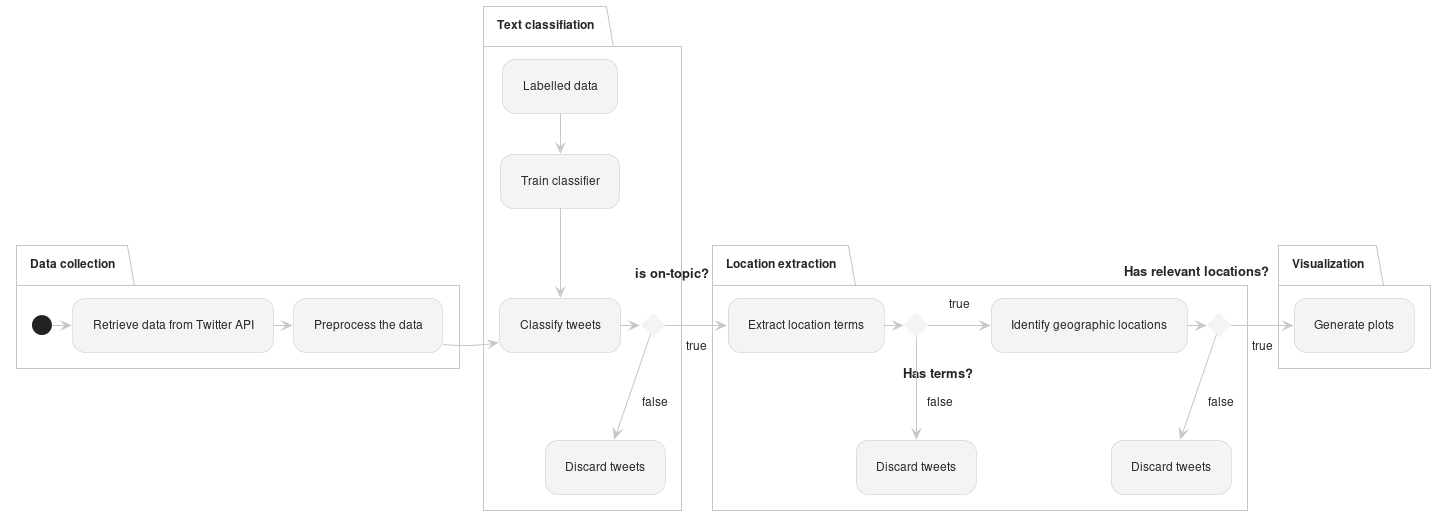
\includegraphics[angle=90, width=\dimexpr\textwidth-11cm\relax, height=\textheight, keepaspectratio]{./images/pipeline.png}
\end{center}
\caption{Flow chart for the pipeline}
\label{fig:flow_chart_big}
\end{figure}

\chapter{Examples}\label{appendix:examples}
\section{Nominatim output example}
 \begin{verbatim}
  {
    "place_id": "100149",
    "licence": "Data © OpenStreetMap contributors, 
                ODbL 1.0. https://osm.org/copyright",
    "osm_type": "node",
    "osm_id": "107775",
    "boundingbox": ["51.3473219", "51.6673219", 
                    "-0.2876474", "0.0323526"],
    "lat": "51.5073219",
    "lon": "-0.1276474",
    "display_name": "London, Greater London, England, 
                     SW1A 2DU, United Kingdom",
    "class": "place",
    "type": "city",
    "importance": 0.9654895765402,
    "icon": "https://nominatim.openstreetmap.org/
             images/mapicons/poi_place_city.p.20.png",
    "address": {
      "city": "London",
      "state_district": "Greater London",
      "state": "England",
      "ISO3166-2-lvl4": "GB-ENG",
      "postcode": "SW1A 2DU",
      "country": "United Kingdom",
      "country_code": "gb"
    },
    "extratags": {
      "capital": "yes",
      "website": "http://www.london.gov.uk",
      "wikidata": "Q84",
      "wikipedia": "en:London",
      "population": "8416535"
    }
  }                           
  \end{verbatim}
                


\end{document}
